\documentclass[border=5pt]{standalone}
\usepackage{tikz}
\usepackage{amsmath}
\usetikzlibrary{positioning, arrows.meta, calc, fit, backgrounds, decorations.pathreplacing}

% --- Color Scheme (Blue-Gray) ---
\definecolor{bgPrimary}{HTML}{DAE8FC}
\definecolor{bgSecondary}{HTML}{E8EEF7}
\definecolor{bgAccent}{HTML}{B3CDE3}
\definecolor{bgInput}{HTML}{F0F4F8}
\definecolor{borderPrimary}{HTML}{6C8EBF}
\definecolor{borderAccent}{HTML}{3A6EA5}
\definecolor{arrowColor}{HTML}{4A6A8A}
\definecolor{textMain}{HTML}{2C3E50}
\definecolor{textLight}{HTML}{7F8C8D}
\definecolor{bgHighlight}{HTML}{FFF3CD}

% --- Styles ---
\tikzset{
  module/.style={draw=borderPrimary, fill=bgPrimary, rounded corners=4pt,
    minimum width=2.8cm, minimum height=1.2cm,
    font=\sffamily\small, text=textMain, line width=0.6pt, align=center},
  novelmodule/.style={draw=borderAccent, fill=bgAccent, rounded corners=4pt,
    minimum width=2.8cm, minimum height=1.2cm,
    font=\sffamily\footnotesize\bfseries, text=textMain, line width=1.0pt, align=center},
  iobox/.style={draw=borderPrimary, fill=bgInput, rounded corners=3pt,
    minimum width=1.8cm, minimum height=0.7cm,
    font=\sffamily\scriptsize, text=textMain, line width=0.5pt, align=center},
  stdarrow/.style={-{Stealth[length=5pt, width=4pt]}, line width=0.6pt, color=arrowColor},
  callout/.style={draw=borderPrimary, fill=bgHighlight, rounded corners=3pt,
    font=\sffamily\scriptsize, text=textMain, inner sep=4pt, line width=0.4pt, align=center},
}

\begin{document}
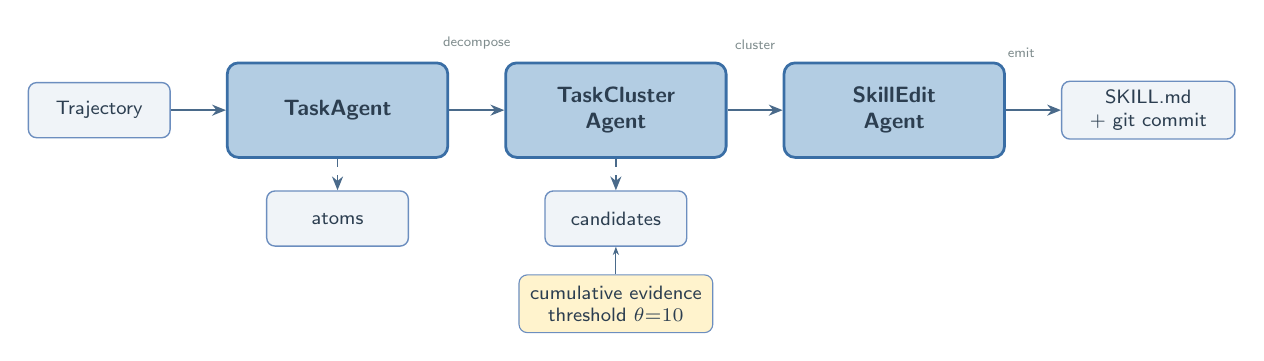
\begin{tikzpicture}

  % === Main flow: horizontal agent chain ===
  \node[iobox] (traj) {Trajectory};

  \node[novelmodule, right=0.7cm of traj] (ta) {TaskAgent};
  \node[novelmodule, right=0.7cm of ta] (tca) {TaskCluster\\Agent};
  \node[novelmodule, right=0.7cm of tca] (sea) {SkillEdit\\Agent};

  \node[iobox, right=0.7cm of sea, minimum width=2.2cm] (out) {SKILL.md\\+ git commit};

  % === Arrows in main flow ===
  \draw[stdarrow] (traj) -- (ta);
  \draw[stdarrow] (ta) -- (tca);
  \draw[stdarrow] (tca) -- (sea);
  \draw[stdarrow] (sea) -- (out);

  % === Data items below agents ===
  \node[iobox, below=0.4cm of ta] (atoms) {atoms};
  \node[iobox, below=0.4cm of tca] (cands) {candidates};

  % Arrows: agents -> data items
  \draw[stdarrow, dashed] (ta.south) -- (atoms.north);
  \draw[stdarrow, dashed] (tca.south) -- (cands.north);

  % === Annotation: cumulative evidence threshold ===
  \node[callout, below=0.35cm of cands, anchor=north] (annot) {%
    cumulative evidence\\
    threshold $\theta{=}10$};
  \draw[-{Stealth[length=3pt]}, arrowColor, line width=0.4pt]
    (annot.north) -- (cands.south);

  % === Arrow labels ===
  \node[above, font=\sffamily\tiny, text=textLight] at ($(ta)!0.5!(tca) + (0, 0.65)$) {decompose};
  \node[above, font=\sffamily\tiny, text=textLight] at ($(tca)!0.5!(sea) + (0, 0.65)$) {cluster};
  \node[above, font=\sffamily\tiny, text=textLight] at ($(sea)!0.5!(out) + (0, 0.55)$) {emit};

\end{tikzpicture}
\end{document}
